\documentclass[../Similarity]{subfiles}
\subsubsection{Temel Benzerlik Teoremi}
\begin{figure}[h!]
    \centering
    \begin{tikzpicture}
        \tkzDefPoint(0,0){A}
        \tkzDefPoint(2,2){C}
        \tkzDefPoint(3,0){B}
        
        \tkzDrawPolygon(A,B,C)
        \tkzDrawPoints(A,B,C)

        \tkzLabelPoints[below left](A)
        \tkzLabelPoints[above](C)
        \tkzLabelPoints[below right](B)

        \tkzLabelSegments[above right](B,C){$a$}
        \tkzLabelSegments[above left](A,C){$b$}
        \tkzLabelSegments[below](A,B){$c$}

        %---------------------------------------------------------------------------------
        
        \tkzDefPoint(6,0){K}
        \tkzDefPoint(8,2){L}
        \tkzDefPoint(9,0){M}
        
        \tkzDrawPolygon(K,M,L)
        \tkzDrawPoints(K,M,L)

        \tkzLabelPoints[below left](K)
        \tkzLabelPoints[above](L)
        \tkzLabelPoints[below right](M)

        \tkzLabelSegments[above right](M,L){$k$}
        \tkzLabelSegments[above left](K,L){$m$}
        \tkzLabelSegments[below](K,M){$l$}


    \end{tikzpicture}
    \caption{Benzer Üçgenler}
    \label{fig:ftosimilarity}
\end{figure}

\ref{fig:ftosimilarity} Benzer üçgenler figüründe de görülebileceği gibi, 
\begin{equation}
    \begin{aligned}    
        \angle A = \angle K\text{, } \angle B = \angle L \text{, } \angle C = \angle M \Leftrightarrow \\
        \frac{a}{k} = \frac{b}{l} = \frac{c}{m} \\
        \widehat{ABC} \sim \widehat{KLM} 
    \end{aligned}
\end{equation}
geçerlidir.